% src/chapter5.tex


\section{觀念與公式}

\subsection{指數的基本概念}
指數表示連乘,$a^n = a \cdot a \cdots a$($n$次),$a > 0$。\\
\textbf{指數律}:
\begin{itemize}
    \item $a^m \cdot a^n = a^{m+n}$
    \item $\frac{a^m}{a^n} = a^{m-n}$
    \item $(a^m)^n = a^{mn}$
    \item $a^{-n} = \frac{1}{a^n}$,$a^{\frac{m}{n}} = \sqrt[n]{a^m}$
\end{itemize}
\textbf{應用}:簡化運算。\\
\textbf{大學技巧}:指數的連續性,$a^x = e^{x \ln a}$。

\subsection{指數函數}
定義:$f(x) = a^x$,$a > 0$且$a \neq 1$。\\
\textbf{性質}:
\begin{itemize}
    \item $a > 1$:單調遞增,$x \to \infty$時$f(x) \to \infty$。
    \item $0 < a < 1$:單調遞減,$x \to \infty$時$f(x) \to 0$。
\end{itemize}
\textbf{應用}:增長模型。\\
\textbf{大學技巧}:微分$\frac{d}{dx} a^x = a^x \ln a$。

\subsection{對數的基本概念}
若$a^x = b$,則$\log_a b = x$,$a > 0$且$a \neq 1$。\\
\textbf{對數律}:
\begin{itemize}
    \item $\log_a (mn) = \log_a m + \log_a n$
    \item $\log_a \left(\frac{m}{n}\right) = \log_a m - \log_a n$
    \item $\log_a (m^n) = n \log_a m$
    \item 換底公式:$\log_a b = \frac{\log_c b}{\log_c a}$
\end{itemize}
\textbf{應用}:化簡複雜運算。\\
\textbf{大學技巧}:自然對數$\ln x$,底$e \approx 2.718$。

\subsection{對數函數}
定義:$f(x) = \log_a x$,$x > 0$。\\
\textbf{性質}:
\begin{itemize}
    \item $a > 1$:單調遞增,過$(1, 0)$。
    \item $0 < a < 1$:單調遞減。
\end{itemize}
\textbf{應用}:壓縮數據。\\
\textbf{大學技巧}:微分$\frac{d}{dx} \log_a x = \frac{1}{x \ln a}$。

\subsection{指數與對數的互逆}
\begin{itemize}
    \item $a^{\log_a x} = x$($x > 0$)
    \item $\log_a (a^x) = x$
\end{itemize}
\textbf{應用}:解方程。\\
\textbf{大學技巧}:泰勒展開,如$\ln(1+x) \approx x - \frac{x^2}{2}$。

\section{例題解析}

\subsection{例題1:指數運算(計算題)}
化簡$2^3 \cdot 2^{-1} \cdot 4^2$。\\
\textbf{解}:$4 = 2^2$,則:
\[
2^3 \cdot 2^{-1} \cdot (2^2)^2 = 2^3 \cdot 2^{-1} \cdot 2^4 = 2^{3-1+4} = 2^6 = 64
\]
\textbf{大學技巧}:用$a^x = e^{x \ln a}$驗算。

\subsection{例題2:對數運算(計算題)}
化簡$\log_2 8 + \log_2 \left(\frac{1}{4}\right)$。\\
\textbf{解}:
\[
\log_2 8 + \log_2 \left(\frac{1}{4}\right) = \log_2 (8 \cdot \frac{1}{4}) = \log_2 2 = 1
\]
\textbf{大學技巧}:換底公式驗證。

\subsection{例題3:解方程(應用題)}
解$3^{x+1} = 27$。\\
\textbf{解}:$27 = 3^3$,則:
\[
3^{x+1} = 3^3 \implies x + 1 = 3 \implies x = 2
\]
或取對數:$\log_3 (3^{x+1}) = \log_3 27$,$x + 1 = 3$。\\
\textbf{大學技巧}:用$\ln$解,$\ln (3^{x+1}) = \ln 27$。

\subsection{例題4:應用問題}
一物質每小時衰減20\%,求半衰期。\\
\textbf{解}:設初量$Q_0$,$Q(t) = Q_0 (0.8)^t$,半衰期時$Q(t) = \frac{Q_0}{2}$:
\[
(0.8)^t = 0.5 \implies t \log 0.8 = \log 0.5 \implies t = \frac{\log 0.5}{\log 0.8} \approx 3.1 \text{小時}
\]
\textbf{大學技巧}:用$\ln$,$t = \frac{\ln 0.5}{\ln 0.8}$。

\section{圖形展示}
指數函數$y = 2^x$與對數函數$y = \log_2 x$:
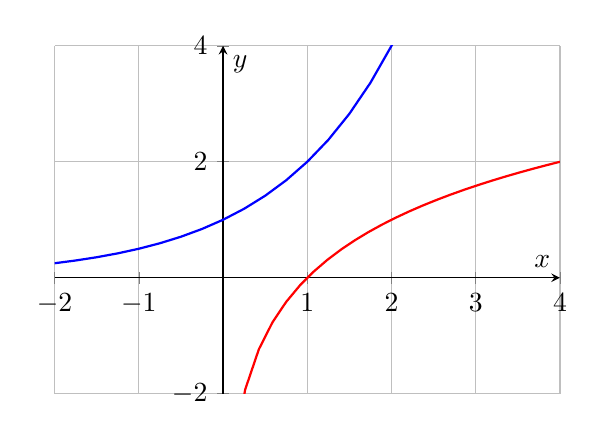
\begin{tikzpicture}
    \begin{axis}[
        axis lines=middle,
        xlabel=$x$,
        ylabel=$y$,
        xmin=-2, xmax=4,
        ymin=-2, ymax=4,
        grid=both,
        width=8cm, height=6cm
    ]
    \addplot[domain=-2:4, blue, thick] {2^x} node[above] {$y = 2^x$};
    \addplot[domain=0.1:4, red, thick] {log2(x)} node[below right] {$y = \log_2 x$};
    \end{axis}
\end{tikzpicture}

\section{題庫}
\begin{enumerate}[label=\arabic*.]
    % 計算題 (10)
    \item 化簡$3^2 \cdot 3^{-3} \cdot 9$。
    \item 計算$\log_4 16$。
    \item 化簡$\log_5 25 + \log_5 125$。
    \item 求$2^{-2} \cdot 8$。
    \item 計算$\log_3 81$。
    \item 化簡$4^{\frac{3}{2}}$。
    \item 求$\log_2 \left(\frac{1}{8}\right)$。
    \item 化簡$10^2 \cdot 10^{-1}$。
    \item 計算$\log_{10} 1000$。
    \item 求$5^0 \cdot 5^3$。
    % 應用題 (10)
    \item 解$2^x = 16$。
    \item 一存款1000元,年利率5\%複利,求5年後金額。
    \item 解$\log_3 (x - 1) = 2$。
    \item 一物質半衰期10小時,求每小時衰減率。
    \item 解$4^{x-1} = 64$。
    \item 若$\log_a 8 = 3$,求$a$。
    \item 一人口每年增長2\%,幾年後翻倍。
    \item 解$\log_2 x + \log_2 (x - 1) = 1$。
    \item 若$pH = -\log_{10} [H^+]$,$[H^+] = 10^{-7}$,求$pH$。
    \item 解$5^{2x} = 125$。
    % 觀念題 (10)
    \item 證$a^{\log_a x} = x$。
    \item 說明指數函數的單調性。
    \item 證$\log_a (mn) = \log_a m + \log_a n$。
    \item 若$a^x = a^y$,則$x, y$關係為何?
    \item 說明對數函數的定義域。
    \item 證$\log_a \left(\frac{m}{n}\right) = \log_a m - \log_a n$。
    \item 若$\log_a b = c$,則$b$如何表示?
    \item 說明換底公式的推導。
    \item 指數函數與對數函數的圖形關係為何?
    \item 若$a > 1$,$\log_a x$的範圍為何?
    % 進階題 (10)
    \item 解$2^{x+1} = 3$(近似值)。
    \item 若$\log_2 x = 3 + \log_2 (x-1)$,求$x$。
    \item 求$3^x$在$x = 2$的泰勒展開(至一階)。
    \item 解$10^{2x-1} = 100$。
    \item 若$\log_a 5 + \log_a 2 = 1$,求$a$。
    \item 求一物質衰減率0.1/小時,半衰期。
    \item 解$2^x + 2^{-x} = 5$。
    \item 若$\log_3 (x^2) = 4$,求$x$。
    \item 解$\log_5 (x+1) - \log_5 (x-1) = 2$。
    \item 若$y = \ln x$,求$x = 1$時斜率。
    % 挑戰題 (20)
    \item 解$3^{x+2} = 5^{x-1}$(近似值)。
    \item 若$\log_2 (x+1) + \log_2 (x-1) = 3$,求$x$。
    \item 求$\ln (1+x)$在$x = 0$的泰勒展開(至三階)。
    \item 解$4^x - 2^x = 3$。
    \item 若$\log_a 3 = 0.5$,求$a$。
    \item 一物質每小時衰減至前值的$\frac{1}{3}$,求半衰期。
    \item 解$2^{2x} - 5 \cdot 2^x + 4 = 0$。
    \item 若$\log_2 (x+2) = 2 + \log_2 x$,求$x$。
    \item 解$\log_3 (x-2) + \log_3 (x+2) = 2$。
    \item 若$y = 2^x$,求$x = 0$時斜率。
    \item 解$5^x = 2^{x+1}$(近似值)。
    \item 若$\log_{10} x = 2 - \log_{10} (x-1)$,求$x$。
    \item 求$e^x$在$x = 0$的泰勒展開(至二階)。
    \item 解$3^{x-1} + 3^{1-x} = 10$。
    \item 若$\log_a 4 = 2 \log_a 2$,求$a$。
    \item 一人口首年1000,每年增長10\%,求10年後人口。
    \item 解$2^x - 2^{-x} = 1$。
    \item 若$\log_5 (x^2 - 1) = 2$,求$x$。
    \item 解$\log_2 (x+3) - \log_2 (x-1) = 3$。
    \item 若$y = \log_3 x$,求$x = 9$時斜率。
\end{enumerate}

